\documentclass[letterpaper, reqno,11pt]{article}
\usepackage[margin=1.0in]{geometry}
\usepackage{color,latexsym,amsmath,amssymb,graphicx,float,listings,tikz,xcolor}
\usepackage{hyperref}

\hypersetup{
colorlinks=true,
linkcolor=magenta,
filecolor=magenta,
urlcolor=cyan,
}

\lstset{
basicstyle=\ttfamily,
columns=fullflexible,
frame=single,
breaklines=true,
postbreak=\mbox{\textcolor{red}{$\hookrightarrow$}\space},
}

\graphicspath{ {images/} }

\begin{document}

\begin{titlepage}
\newgeometry{margin=3cm}
\centering

\vspace*{\stretch{2}}

\Large Investigation of HeNe Laser Emission Spectra

\normalsize

\vspace{\stretch{1}}

% \normalsize Power Supplies and Voltage Regulators

\vspace{\stretch{0.5}}

\begin{tabular}{ll}
Name & Xander Naumenko \\[2ex]
Student number & 38198354 \\[2ex]
Partner & Renu Rajamagesh \\[2ex]
Lab name & Fourier optics \\[2ex]
Lab station  & L2C \\[2ex]
Assigned TA            & Rachel Wang, Mahdi Rabiel \\[2ex]
Lab \#            & 2 \\[2ex]
Notes &  N/A
\end{tabular}

\vspace{\stretch{1}}

\begin{abstract}
    HeNe lasers are one relatively easy way of creating a laser beam for general optics uses. In this lab we investigate the properties and operating conditions of such lasers. Specifically, the stability conditions of the lasing and the spectral emissions of the HeNe were analyzed thoroughly to get a clear picture of the underlying mechanics causing the laser's production. The biggest result is that, using an op-amp, the spectral difference between lasing and non-lasing HeNe was recorded to have peaks at the atomic frequencies of the laser.
\end{abstract}

\vspace{\stretch{2}}
\end{titlepage}

\newpage

\section{Research Note}

\subsection{Introduction}

When set up in a cavity, stimulated emission causes excited HeNe gas to emit a laser at a frequency of 632.8nm. When such lasing occurs the emission spectrum of the gas also changes slightly due to a shift in occupied energy levels. A study was conducted to determine the exact nature of this emission spectrum change. The theoretical frequencies lines that share similar energy levels with 632.8nm laser were recovered successfully.

\subsection{Methods}

A HeNe laser was obtained using the gas, and electrode and two concave mirrors. Using a series of mirrors, the emission of the gas itself was directed to a monochromator. By using a spinning disk to periodically start at stop the lasing process and connecting the output of the monochromator to a lock-in amplifier, a high resolution measurement of the change in emission spectrum between lasing and no lasing was obtained.

\subsection{Results}

See figure \ref{fig:rn} for the change in emission spectrum caused by the lasing process. The frequencies that had the largest modulation were 594.5nm, 607.4nm and 609.6nm. From a theoretical standpoint, this makes sense. Using NIST data, the lower energy level of the 632.8nm lasing process is $150858\text{cm}^{-1}$, which is the upper energy level of the 594.5nm and 609.6nm transitions. The upper energy level of $607.4$nm is $150917\text{cm}^{-1}$, which while not exactly the same, is close enough that it is also modulated by the lasing process (although as seen by the graph it is to a lower extent).

The process by which this modulation occurs is that when lasing occurs, the 632.8 transition becomes amplified significantly. This results in many atoms with energies the bottom of its transition level. This larger than previously number of atoms then spontaneously emit, causing the modulation seen experimentally. 

\begin{figure}[htpb]
    \centering
    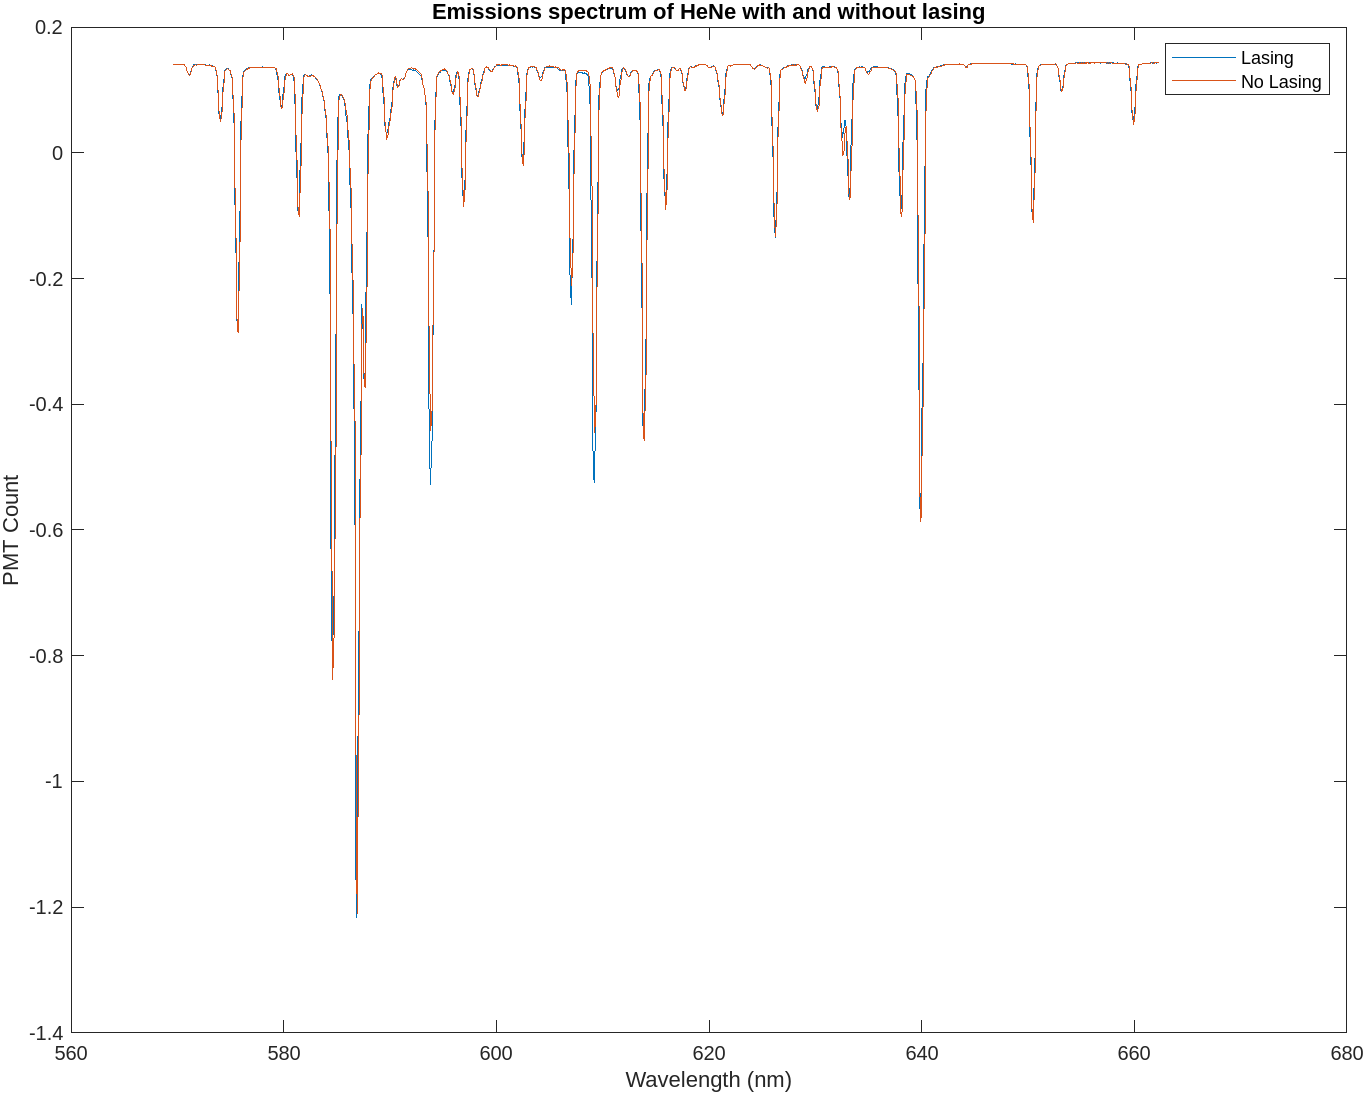
\includegraphics[width=0.45\textwidth]{4A}
    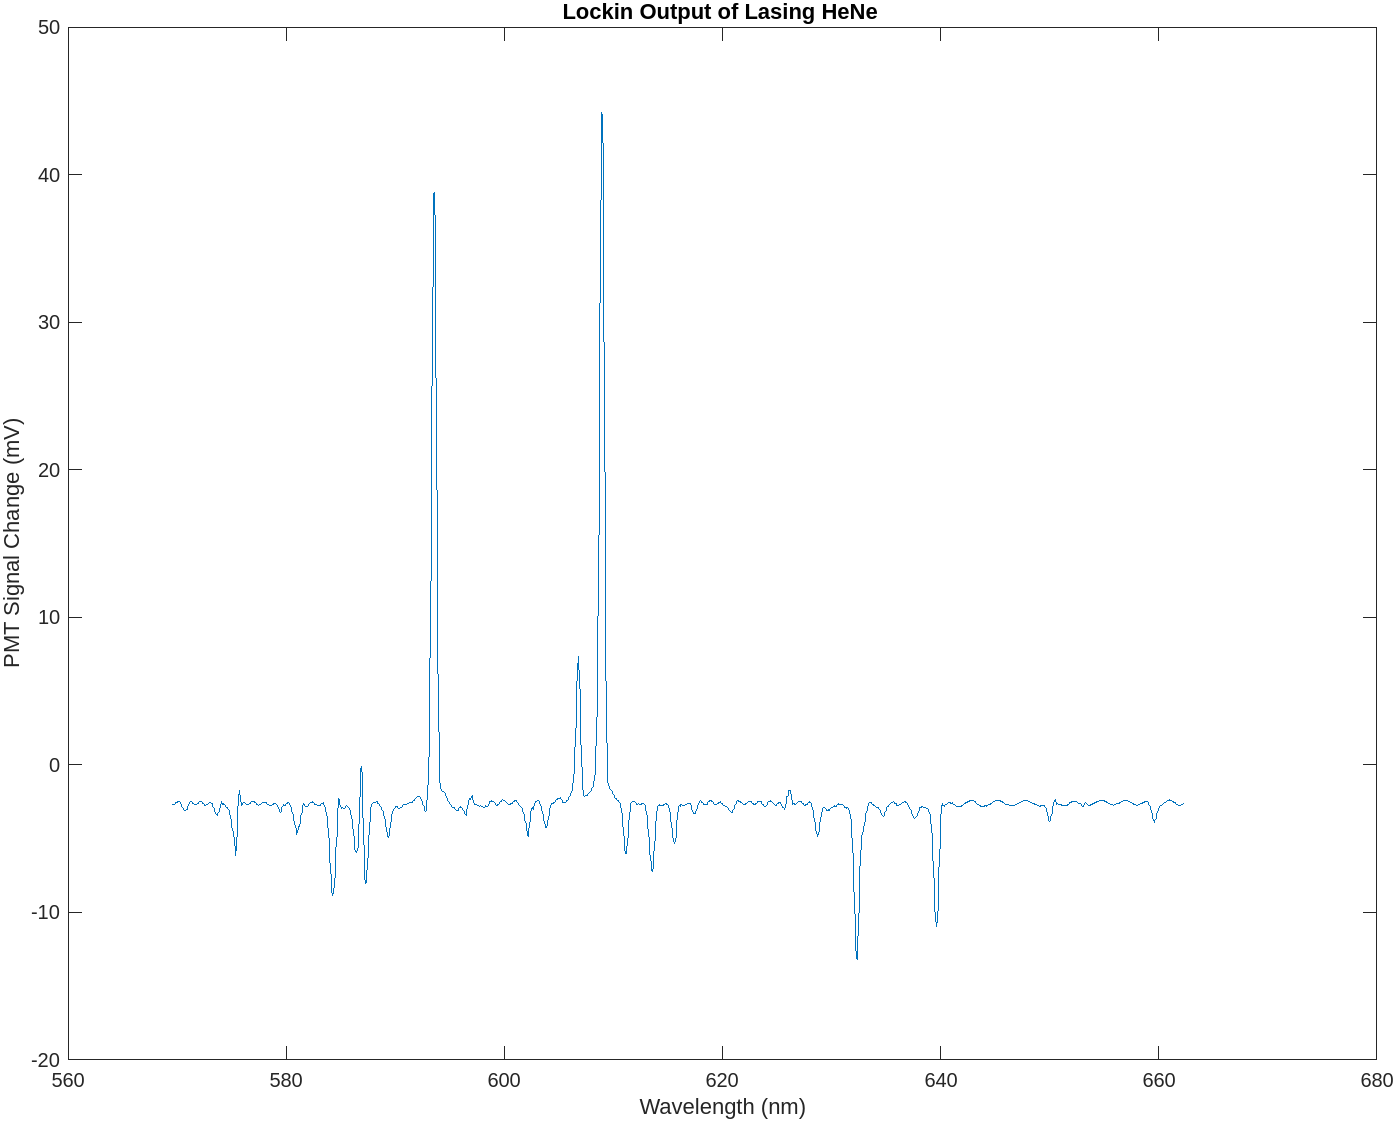
\includegraphics[width=0.45\textwidth]{4F}
    \caption{Emission spectrum between lasing and unstimulated HeNe gas (left) and a higher resolution difference between the two collected using an op-amp (right).}
    \label{fig:rn}
\end{figure}

\newpage

\section{2.3.1: Laser Alignment and Stability}

\noindent \textcolor{red}{2.3.1A.} The stability conditions for lasing, as described in the appendix are:
\[
0\leq \left(1+ \frac{d}{R_1}\right) \left( 1+ \frac{d}{R_2} \right) \leq 1
.\]
In our case, $R_2=\infty$, so this reduces to $0\leq 1+ \frac{d}{R_1}\leq 1$. Assuming $R_1$ is concave (so $R_1< 0$), this gives $d=-R_1$.

To measure this, we first got the HeNe lasing by adjusting the mirror as described in the manual. Then we pushed the mirror back until lasing stopped, and measured the distance from the fixed HR mirror. Experimentally we found this to be $53$cm, so $R_2=-53$cm.

\medskip

\noindent \textcolor{red}{2.3.1B.} With the new mirror, there were four regions (all distances measured relative to HR mirror): at less than 54cm there was lasing, between 54cm and 56.5cm there was none, between 56.5cm and 65cm it lased and then finally disappeared after 65cm. However after 65cm it wasn't entirely consistent, and depending on fine alignment it would sometimes lase farther than that.

These points can be explained theoretically. The first disappearance corresponds to $1+\frac{d}{R_1}=0$, i.e. $d=-R_1$. From part A we'd expect this to be around $53$cm, which our measurement of $54$cm was fairly close to. The reappearance at $56.5$ is for $1+\frac{d}{R_2}=0\implies d=-R_2$. From the box the mirror came in we expect this to be $60$cm. One possible reason for this somewhat small discrepancy is just the measurement error, as using a meter stick to estimate exactly where the laser starts can be inconsistent. The final reappearance occurs when
\[
\left(1+ \frac{d}{R_1}\right) \left( 1+ \frac{d}{R_2} \right) = 1\implies d=-(R_1+R_2)
.\]
Our measured value was 65cm, which was very difference than the expected of 113. In fact, given where the raspberry pi camera was located and the length of the slide we shouldn't have even seen a reappearance at all. The most likely cause for this discrepancy is misalignment of the mirrors. Even if everything else in the setup was perfect, the mirrors have finite size, so a small misalignment could cause the reflected laser to strike outside the mirror when distances are far enough. Something like alignment would also explain the inconsistencies with seeing exactly where the laser reappears. See figure \ref{fig:1A} for the plot and table.

\begin{figure}[htpb]
    \centering
    \begin{minipage}[b]{0.45\textwidth}
    \begin{tabular}{|l|l|l|}
    \hline
    Value & Theoretical & Measured \\
    \hline
    $-R_1$ & 53 & 54 \\
    $-R_2$ & 60 & 56.5 \\
    $-(R_1+R_2)$ & 113 & 65 \\
    \hline
    \end{tabular}
    \caption{Table caption.}
    \label{fig:table1}
    \end{minipage}
    \hfill
    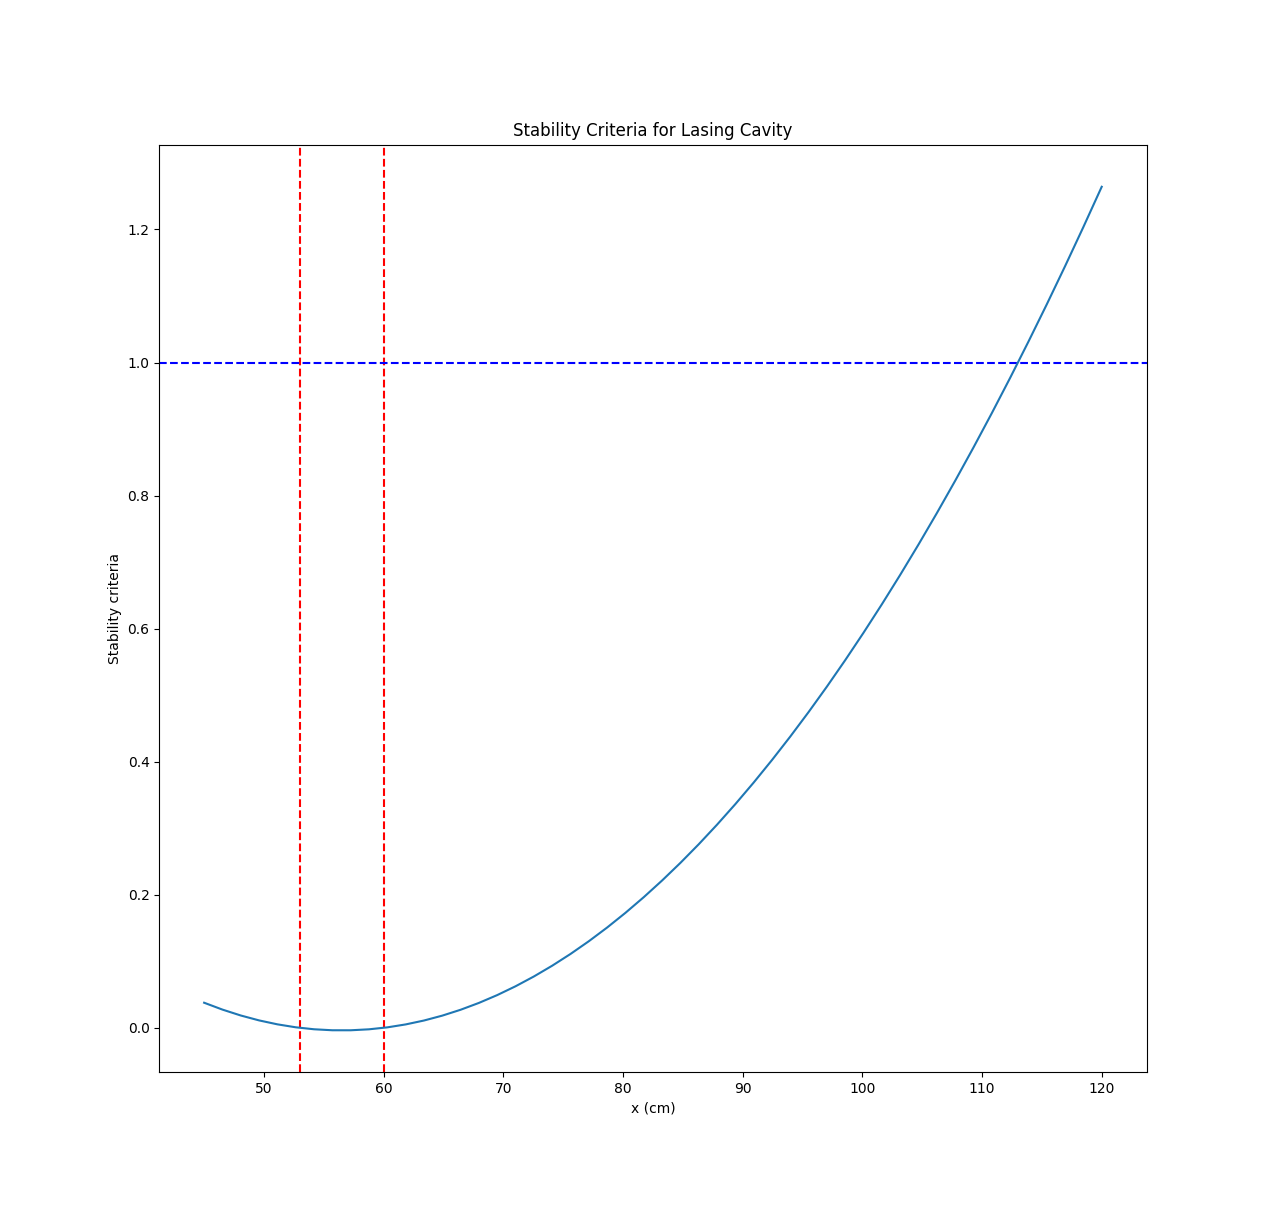
\includegraphics[width=0.5\textwidth]{1B}
    \caption{Plot and table for 2.3.1B. The theoretical values were found from 2.3.1B and the mirror box.}
    \label{fig:1A}
\end{figure}

\noindent \textcolor{blue}{2.3.1i.} You could use a convex mirror, for the calculations let's say for $R_2$ while $R_1$ is still concave. From the condition that $\left(1+ \frac{d}{R_1}\right) \left( 1+ \frac{d}{R_2} \right)\geq 0$ we have that $d<R_1$. From the condition that $\left(1+ \frac{d}{R_1}\right) \left( 1+ \frac{d}{R_2} \right)\leq 1$, we have that $-R_1<R_2$, i.e. the magnitude of the convex mirror's radius of curvature must be greater than that of the concave mirror.

\noindent \textcolor{red}{2.3.2A.} See figure \ref{fig:2A} for some of the observed nodes. The highest order node observed was Hermite-Gaussian TEM$_{22}$, see the figure for explanations.

\begin{figure}[tb]
    \centering
    \includegraphics[width=0.3\textwidth]{data/2A/im_0228_20240301_175138.jpg}
    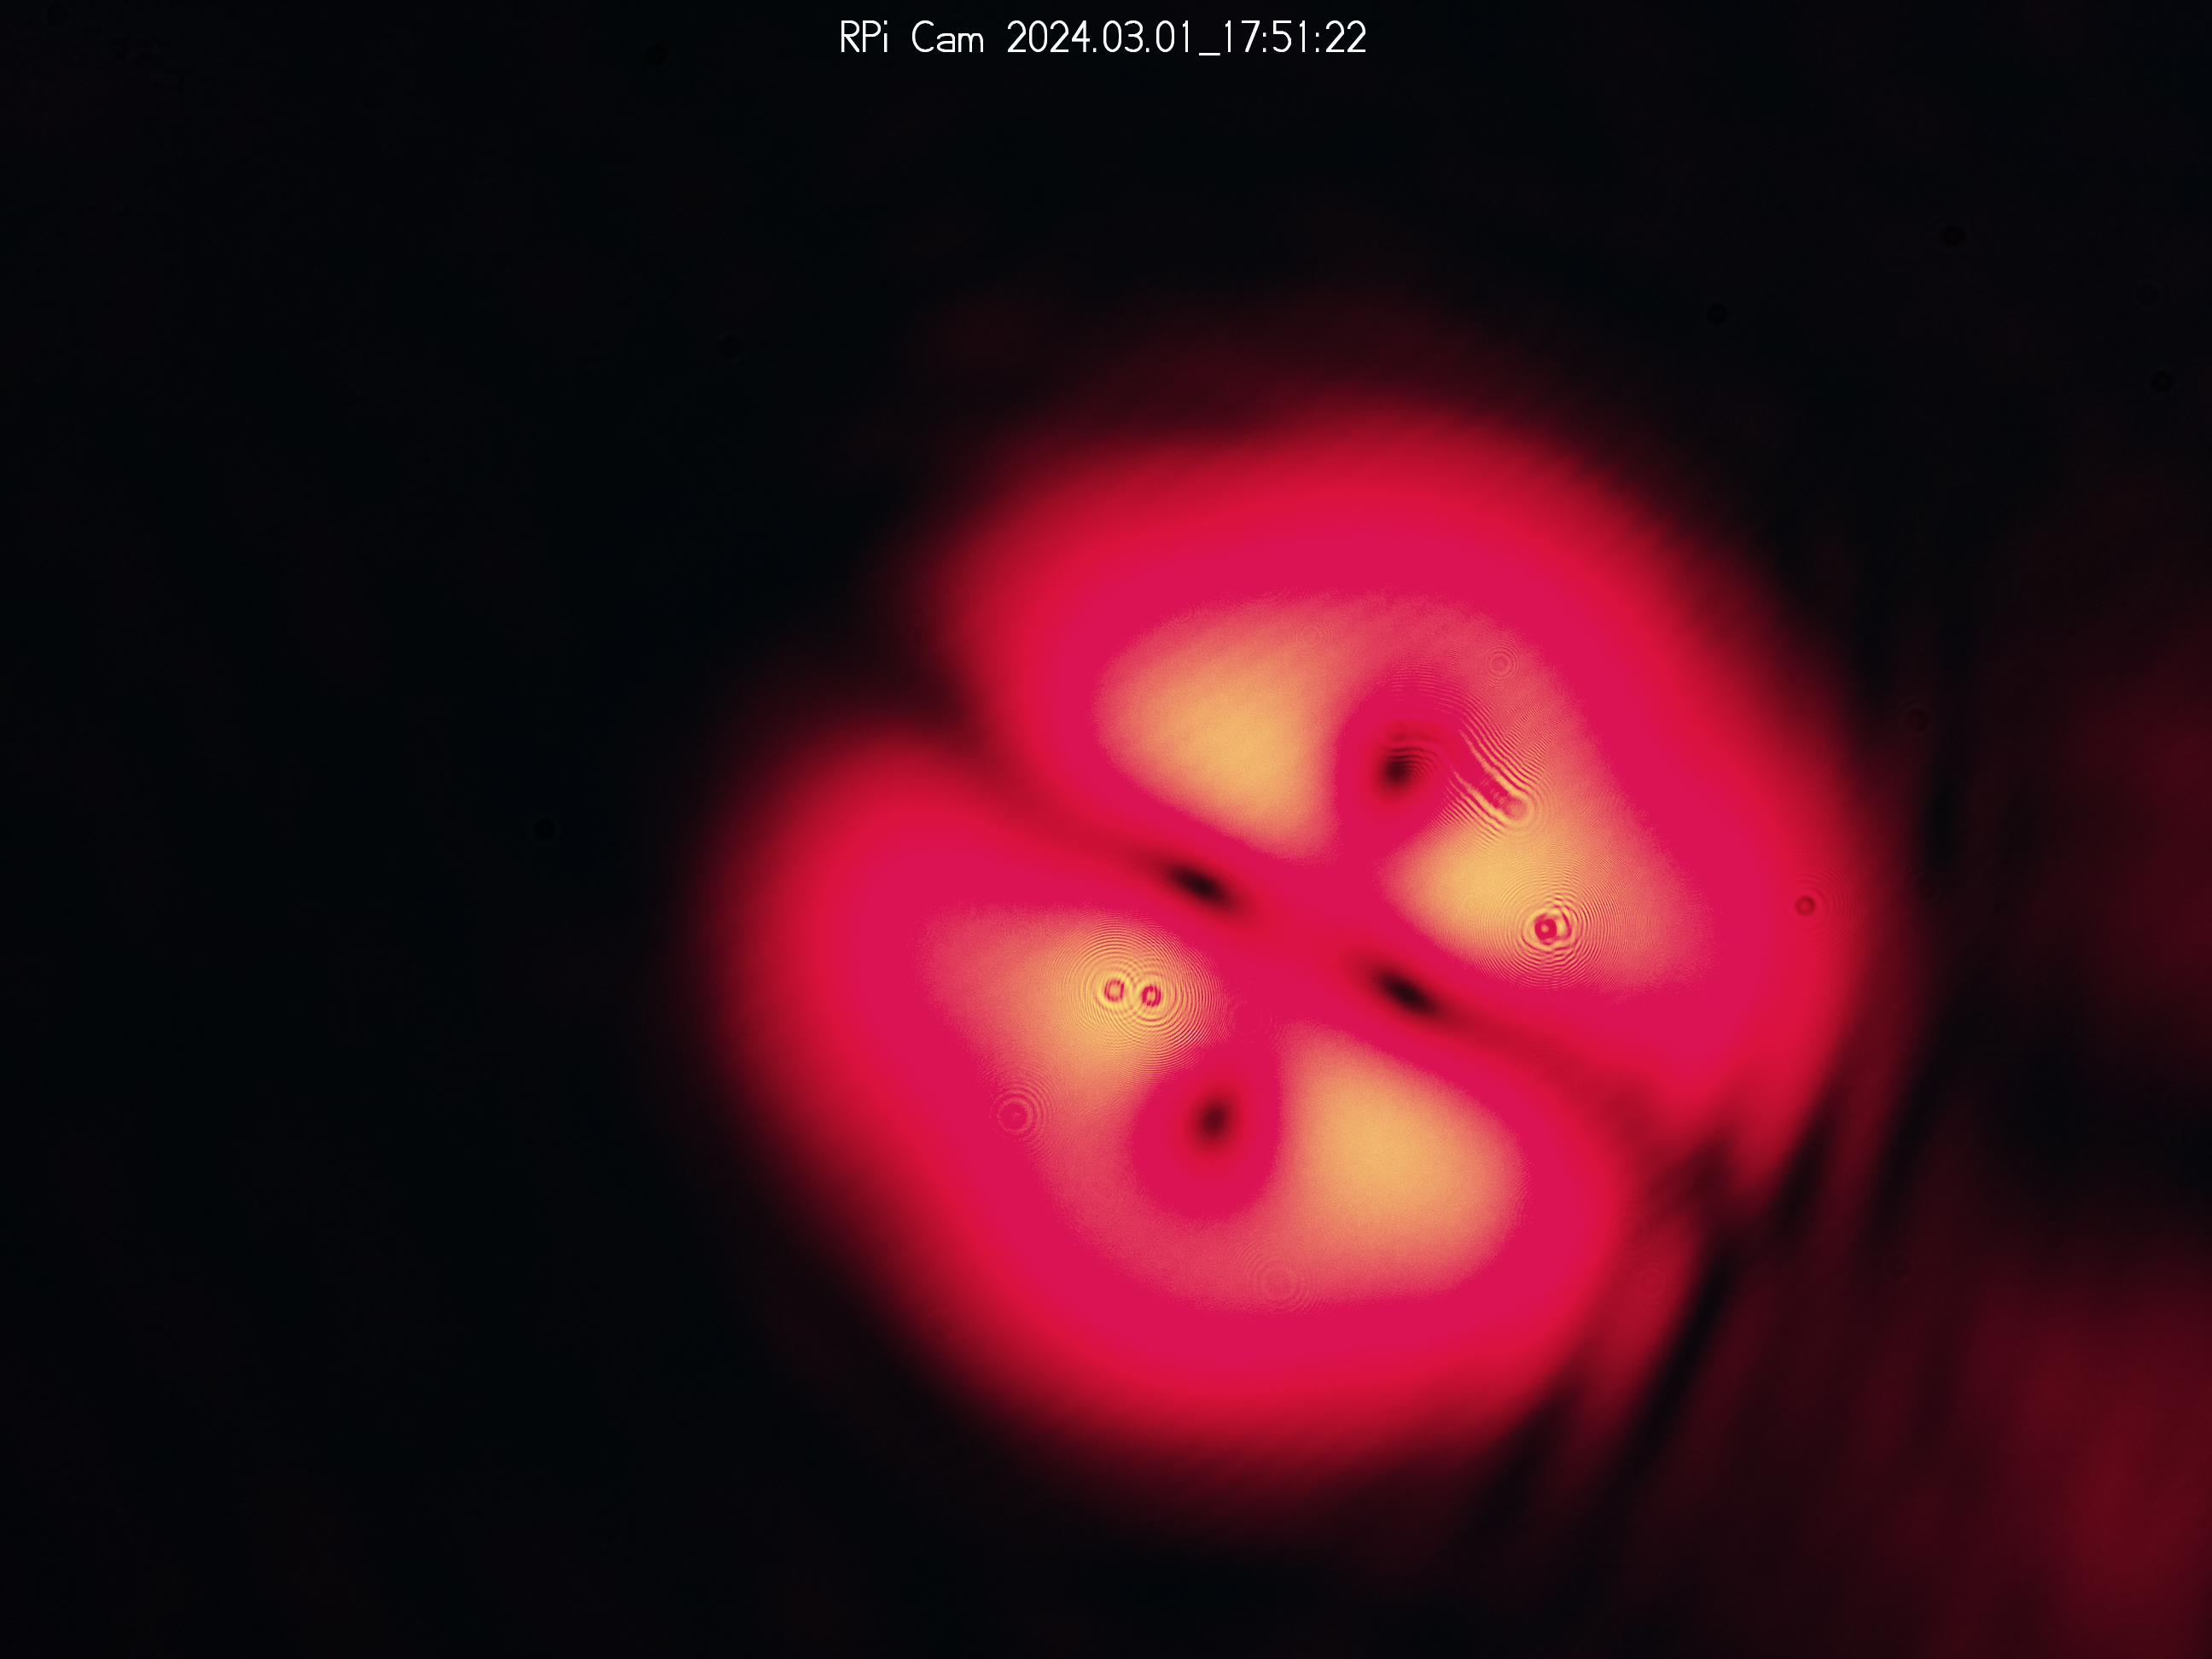
\includegraphics[width=0.3\textwidth]{data/2A/im_0224_20240301_175122.jpg}
    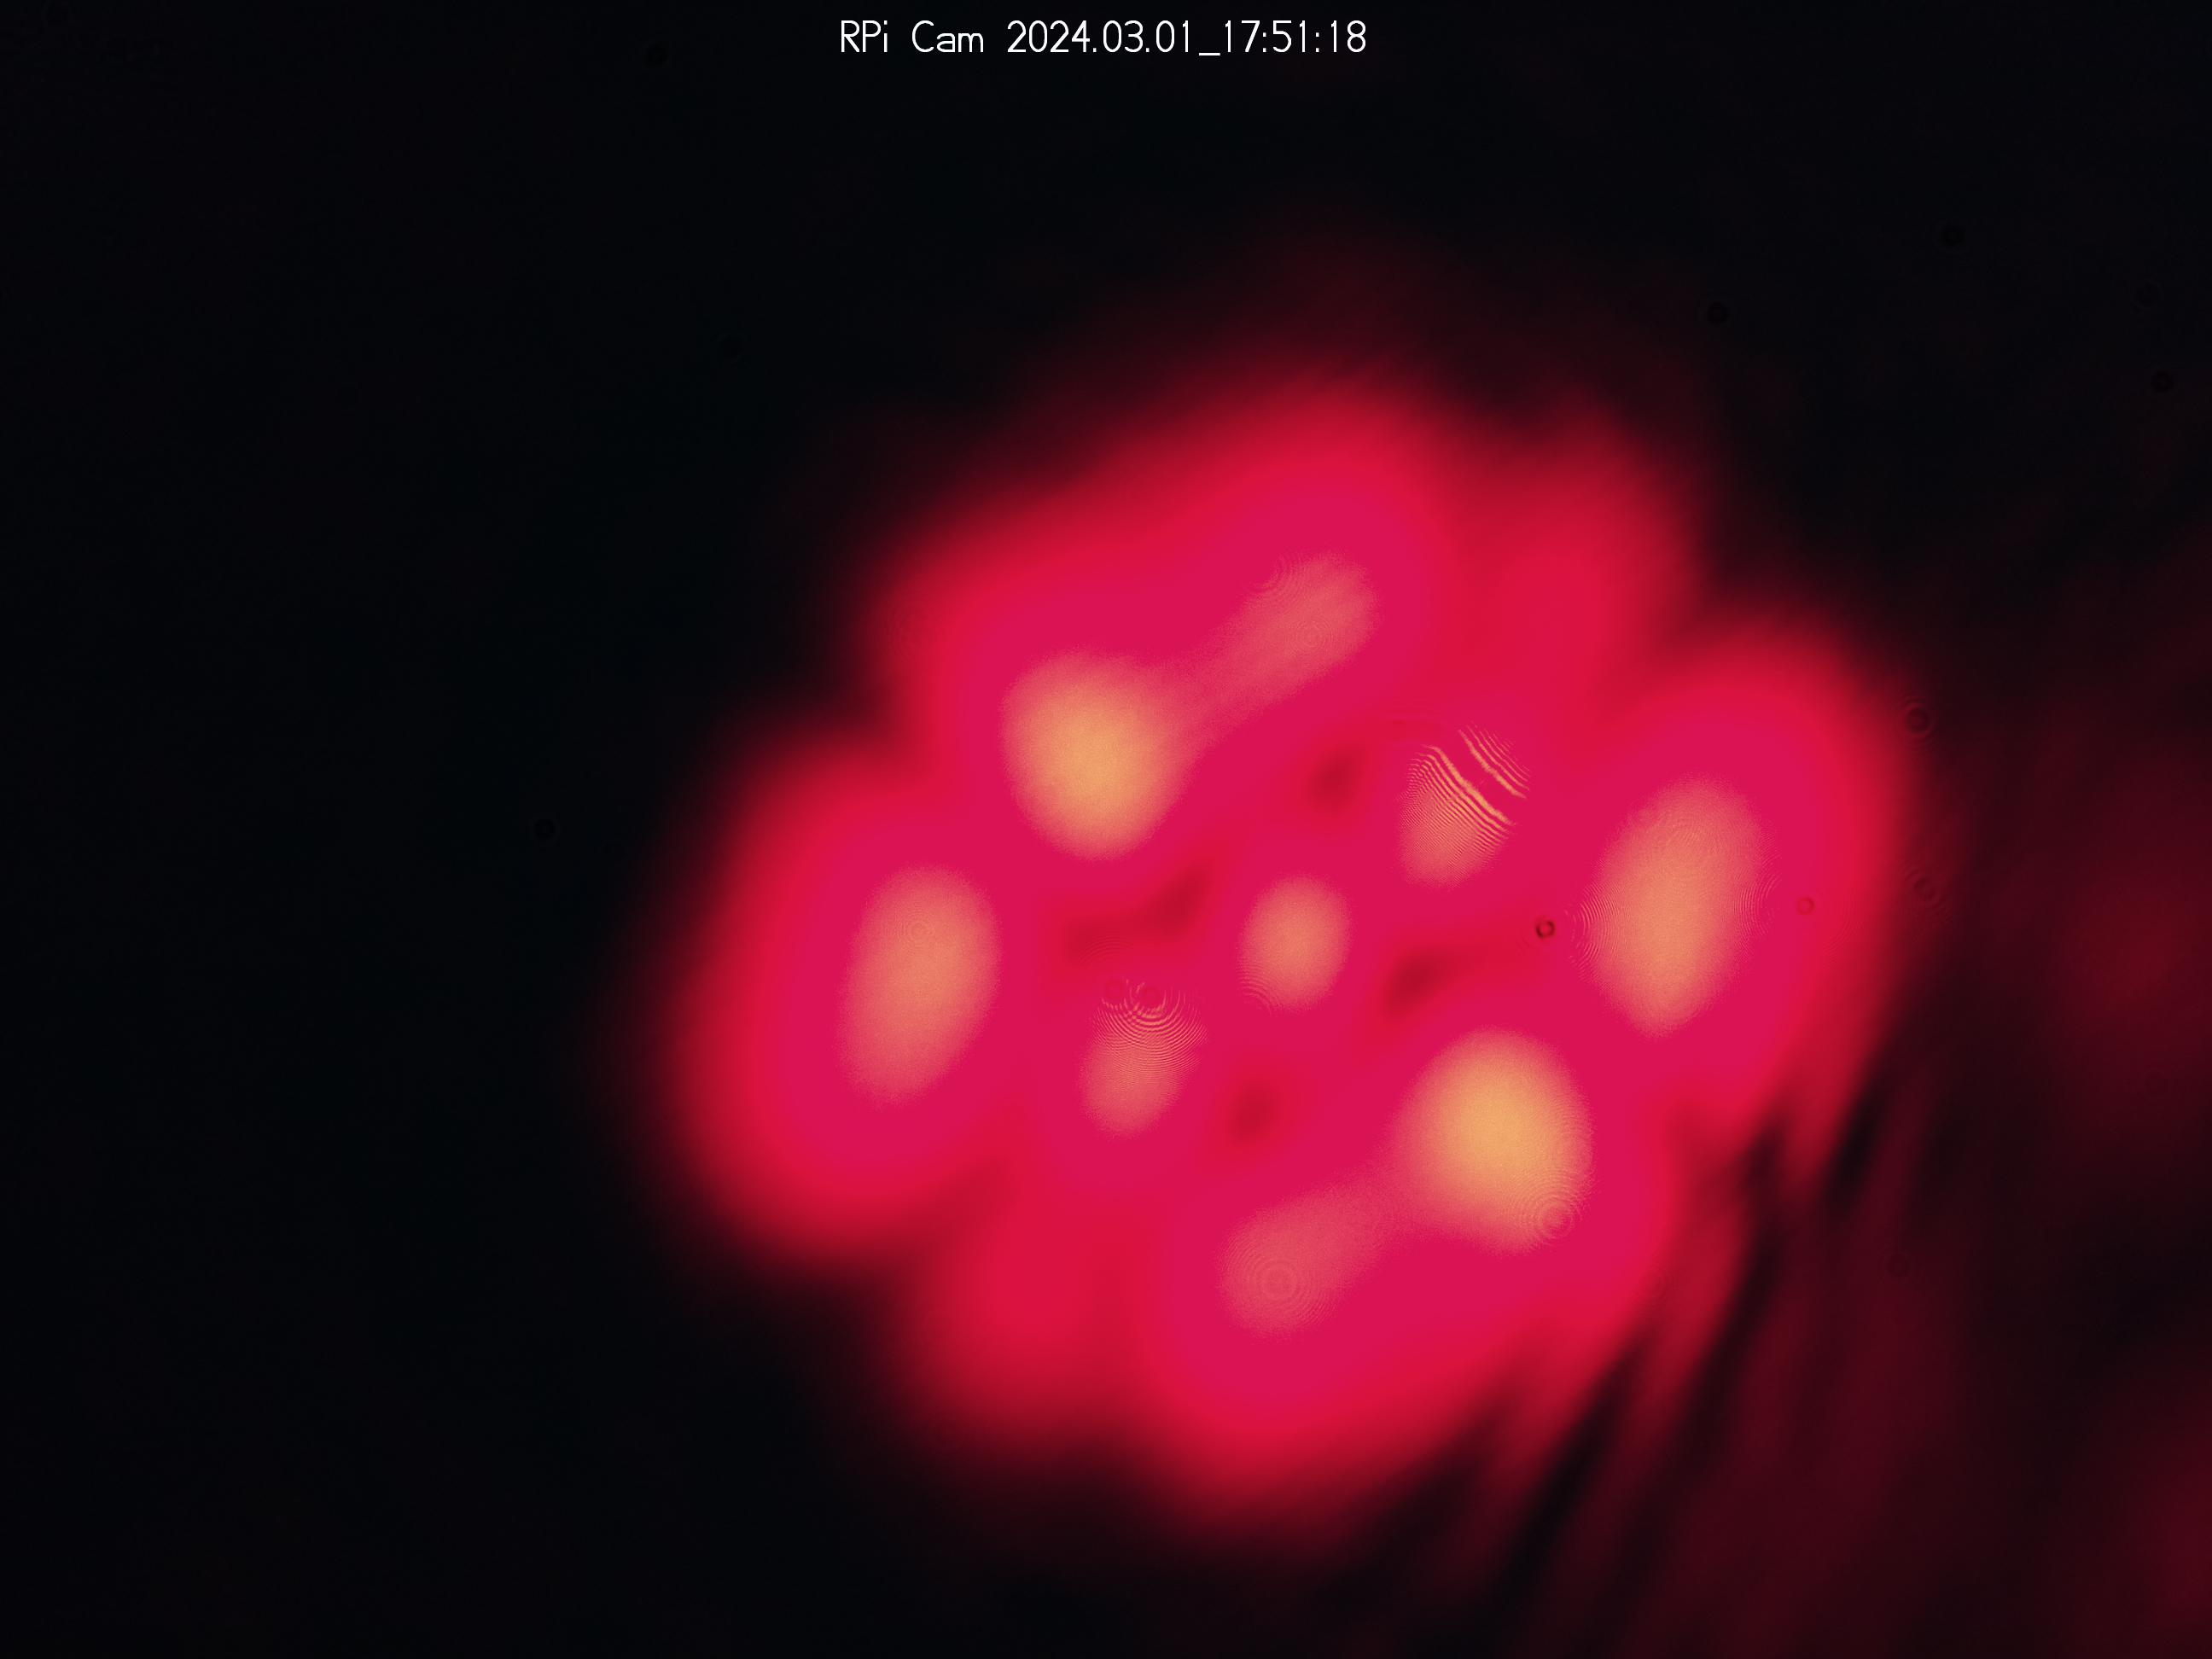
\includegraphics[width=0.3\textwidth]{data/2A/im_0223_20240301_175118.jpg}
    \caption{Selection of mode profiles seen. Left is TEM$_{00}$, middle is TEM$_{11}$ and right is TEM$_{22}$, all Hermite-Gaussian. Especially the TEM$_{22}$ features are fairly blurry, this could either be from interference with other nodes, or just the focus in the camera not being perfectly set up. All of these pictures were taken with a cavity length of 36.5cm.}
    \label{fig:2A}
\end{figure}

\noindent \textcolor{red}{2.3.2B.} See figure \ref{fig:2B}. We started with the TEM$_{22}$ mode, and as can be seen in the figure the modes decreased in complexity until we reached the TEM$_{00}$ mode. This can be explained by the nature of stimulated emission. When a light passes through the HeNe and causes stimulated emission, the resulting photon is in the exact same mode as the first. Therefore if any light is blocked during lasing, this causes an exponential suppression of that mode. By closing the iris, any modes with any light in these higher modes (which is further away from the center of the beam) are suppressed, so by the time the iris is small enough only the TEM$_{00}$ mode remains.

\begin{figure}[htpb]
    \centering
    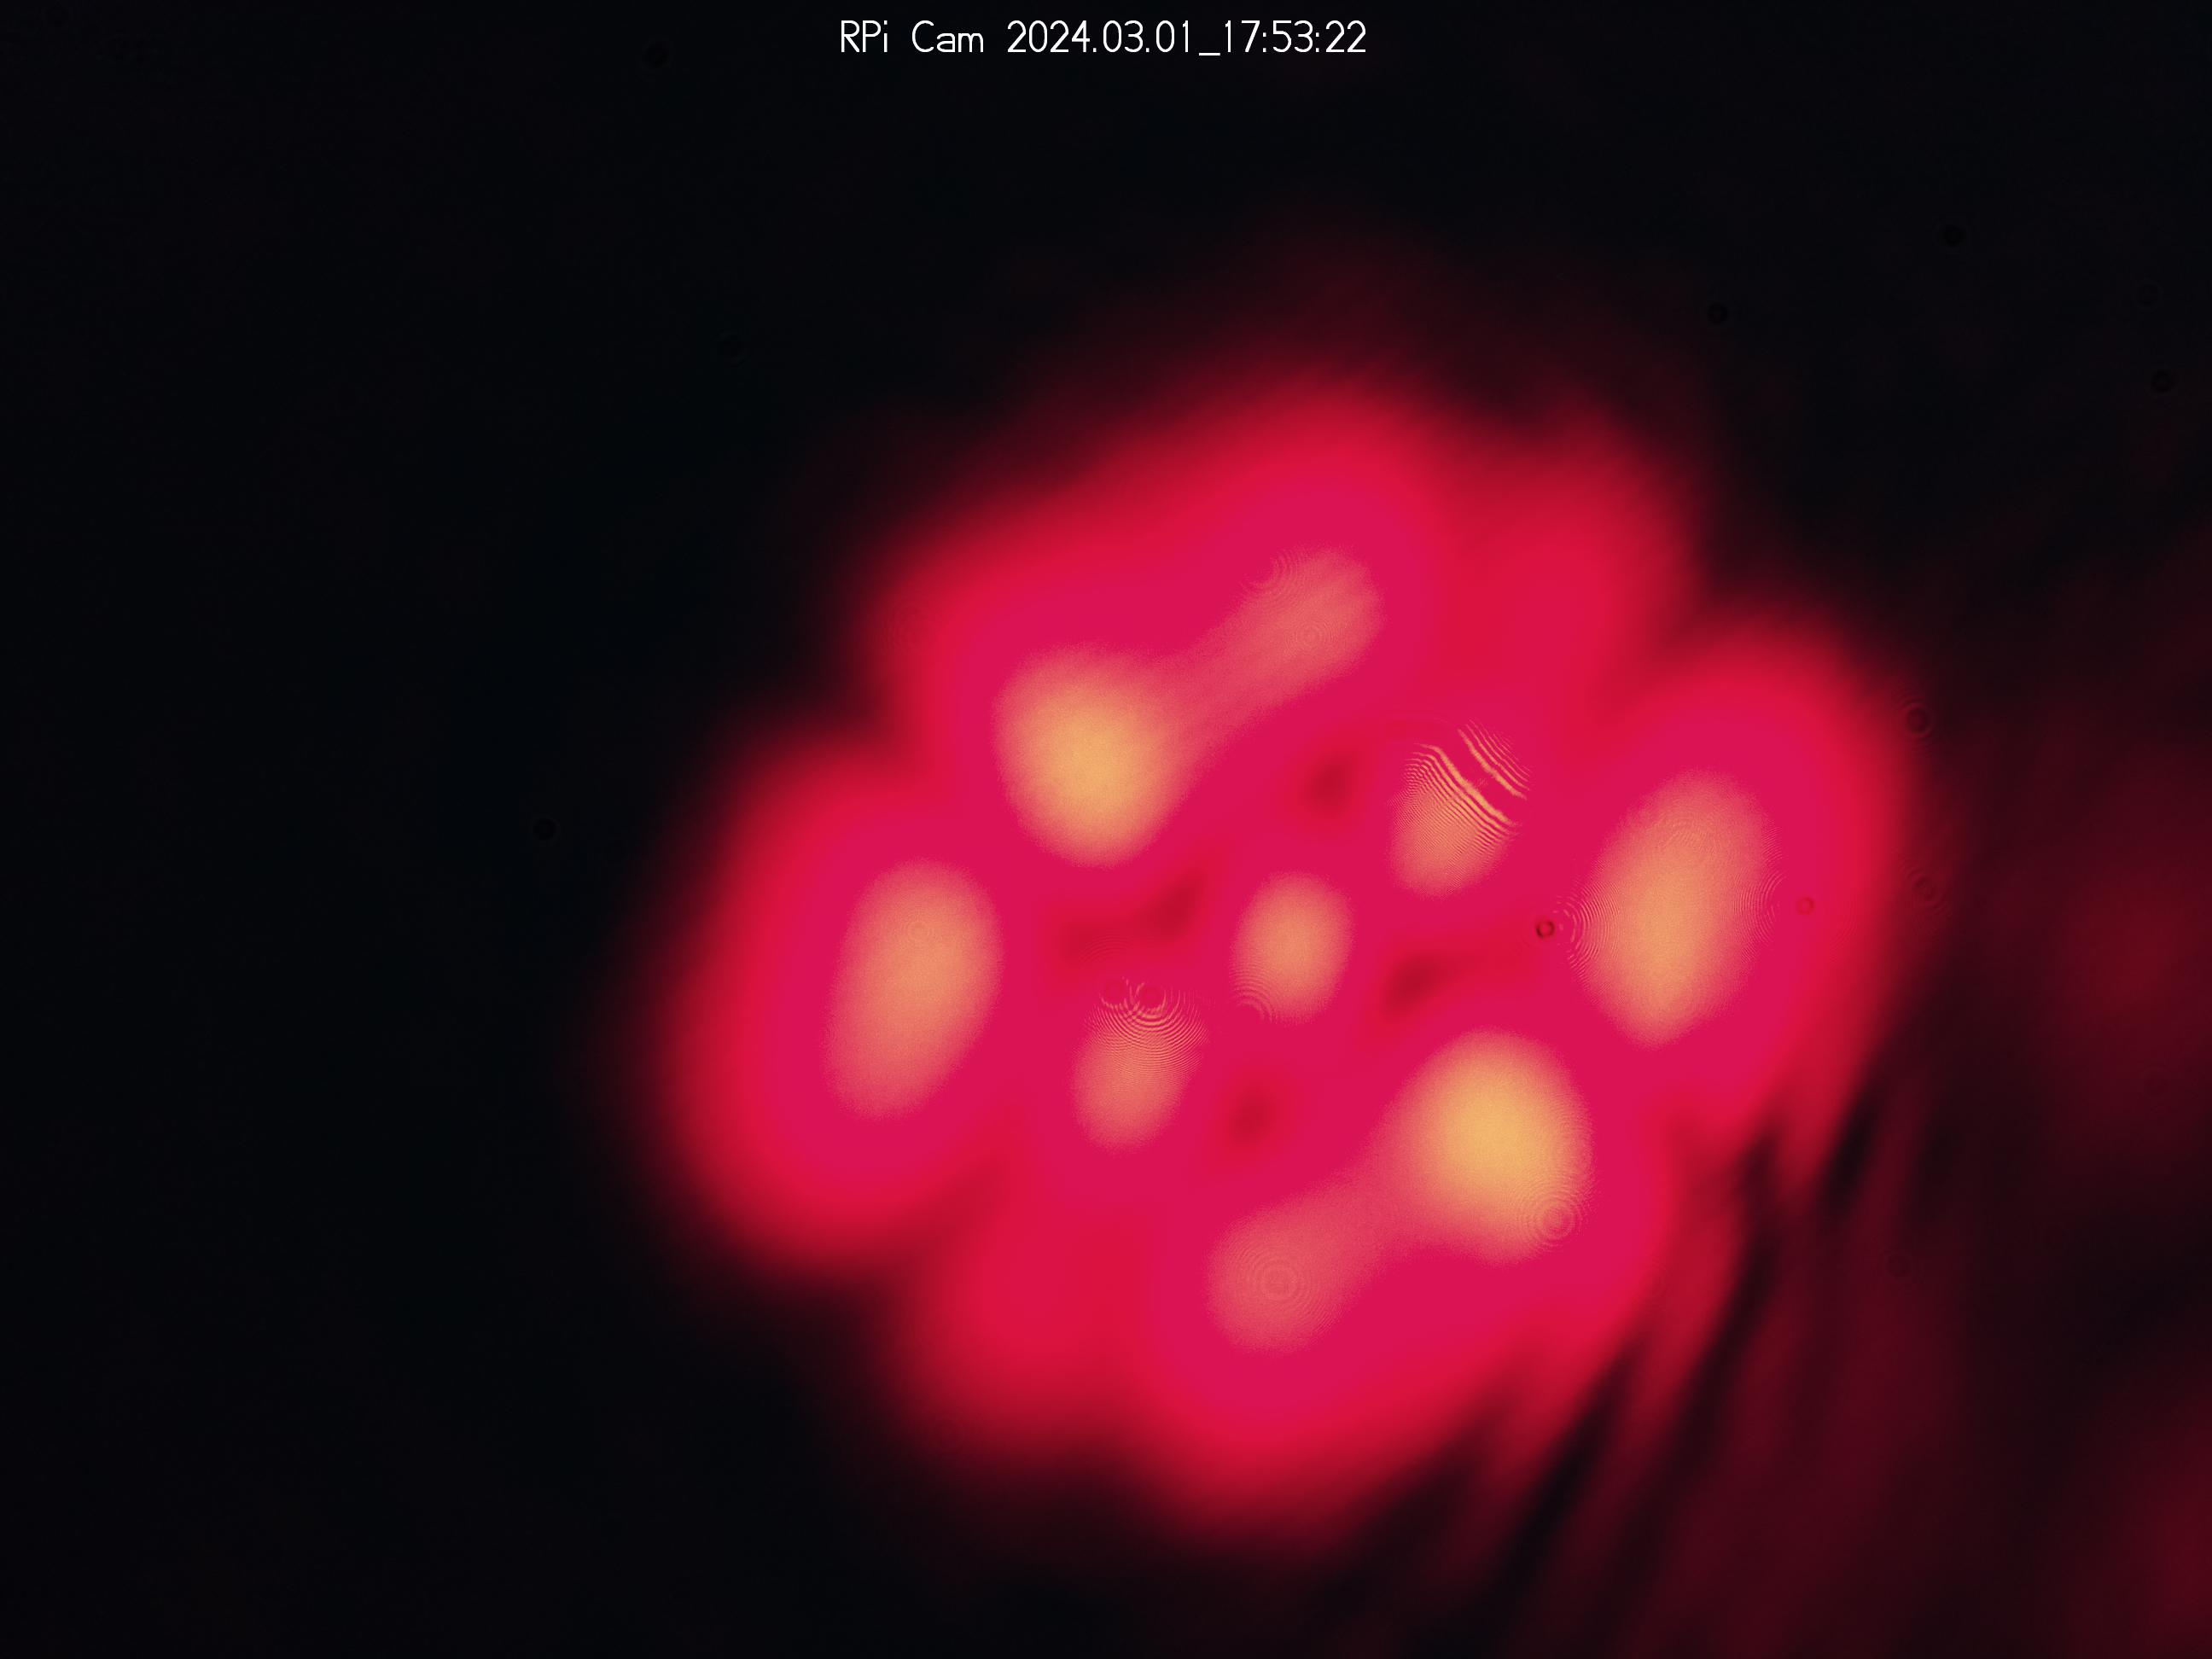
\includegraphics[width=0.3\textwidth]{data/2B/im_0229_20240301_175322.jpg}
    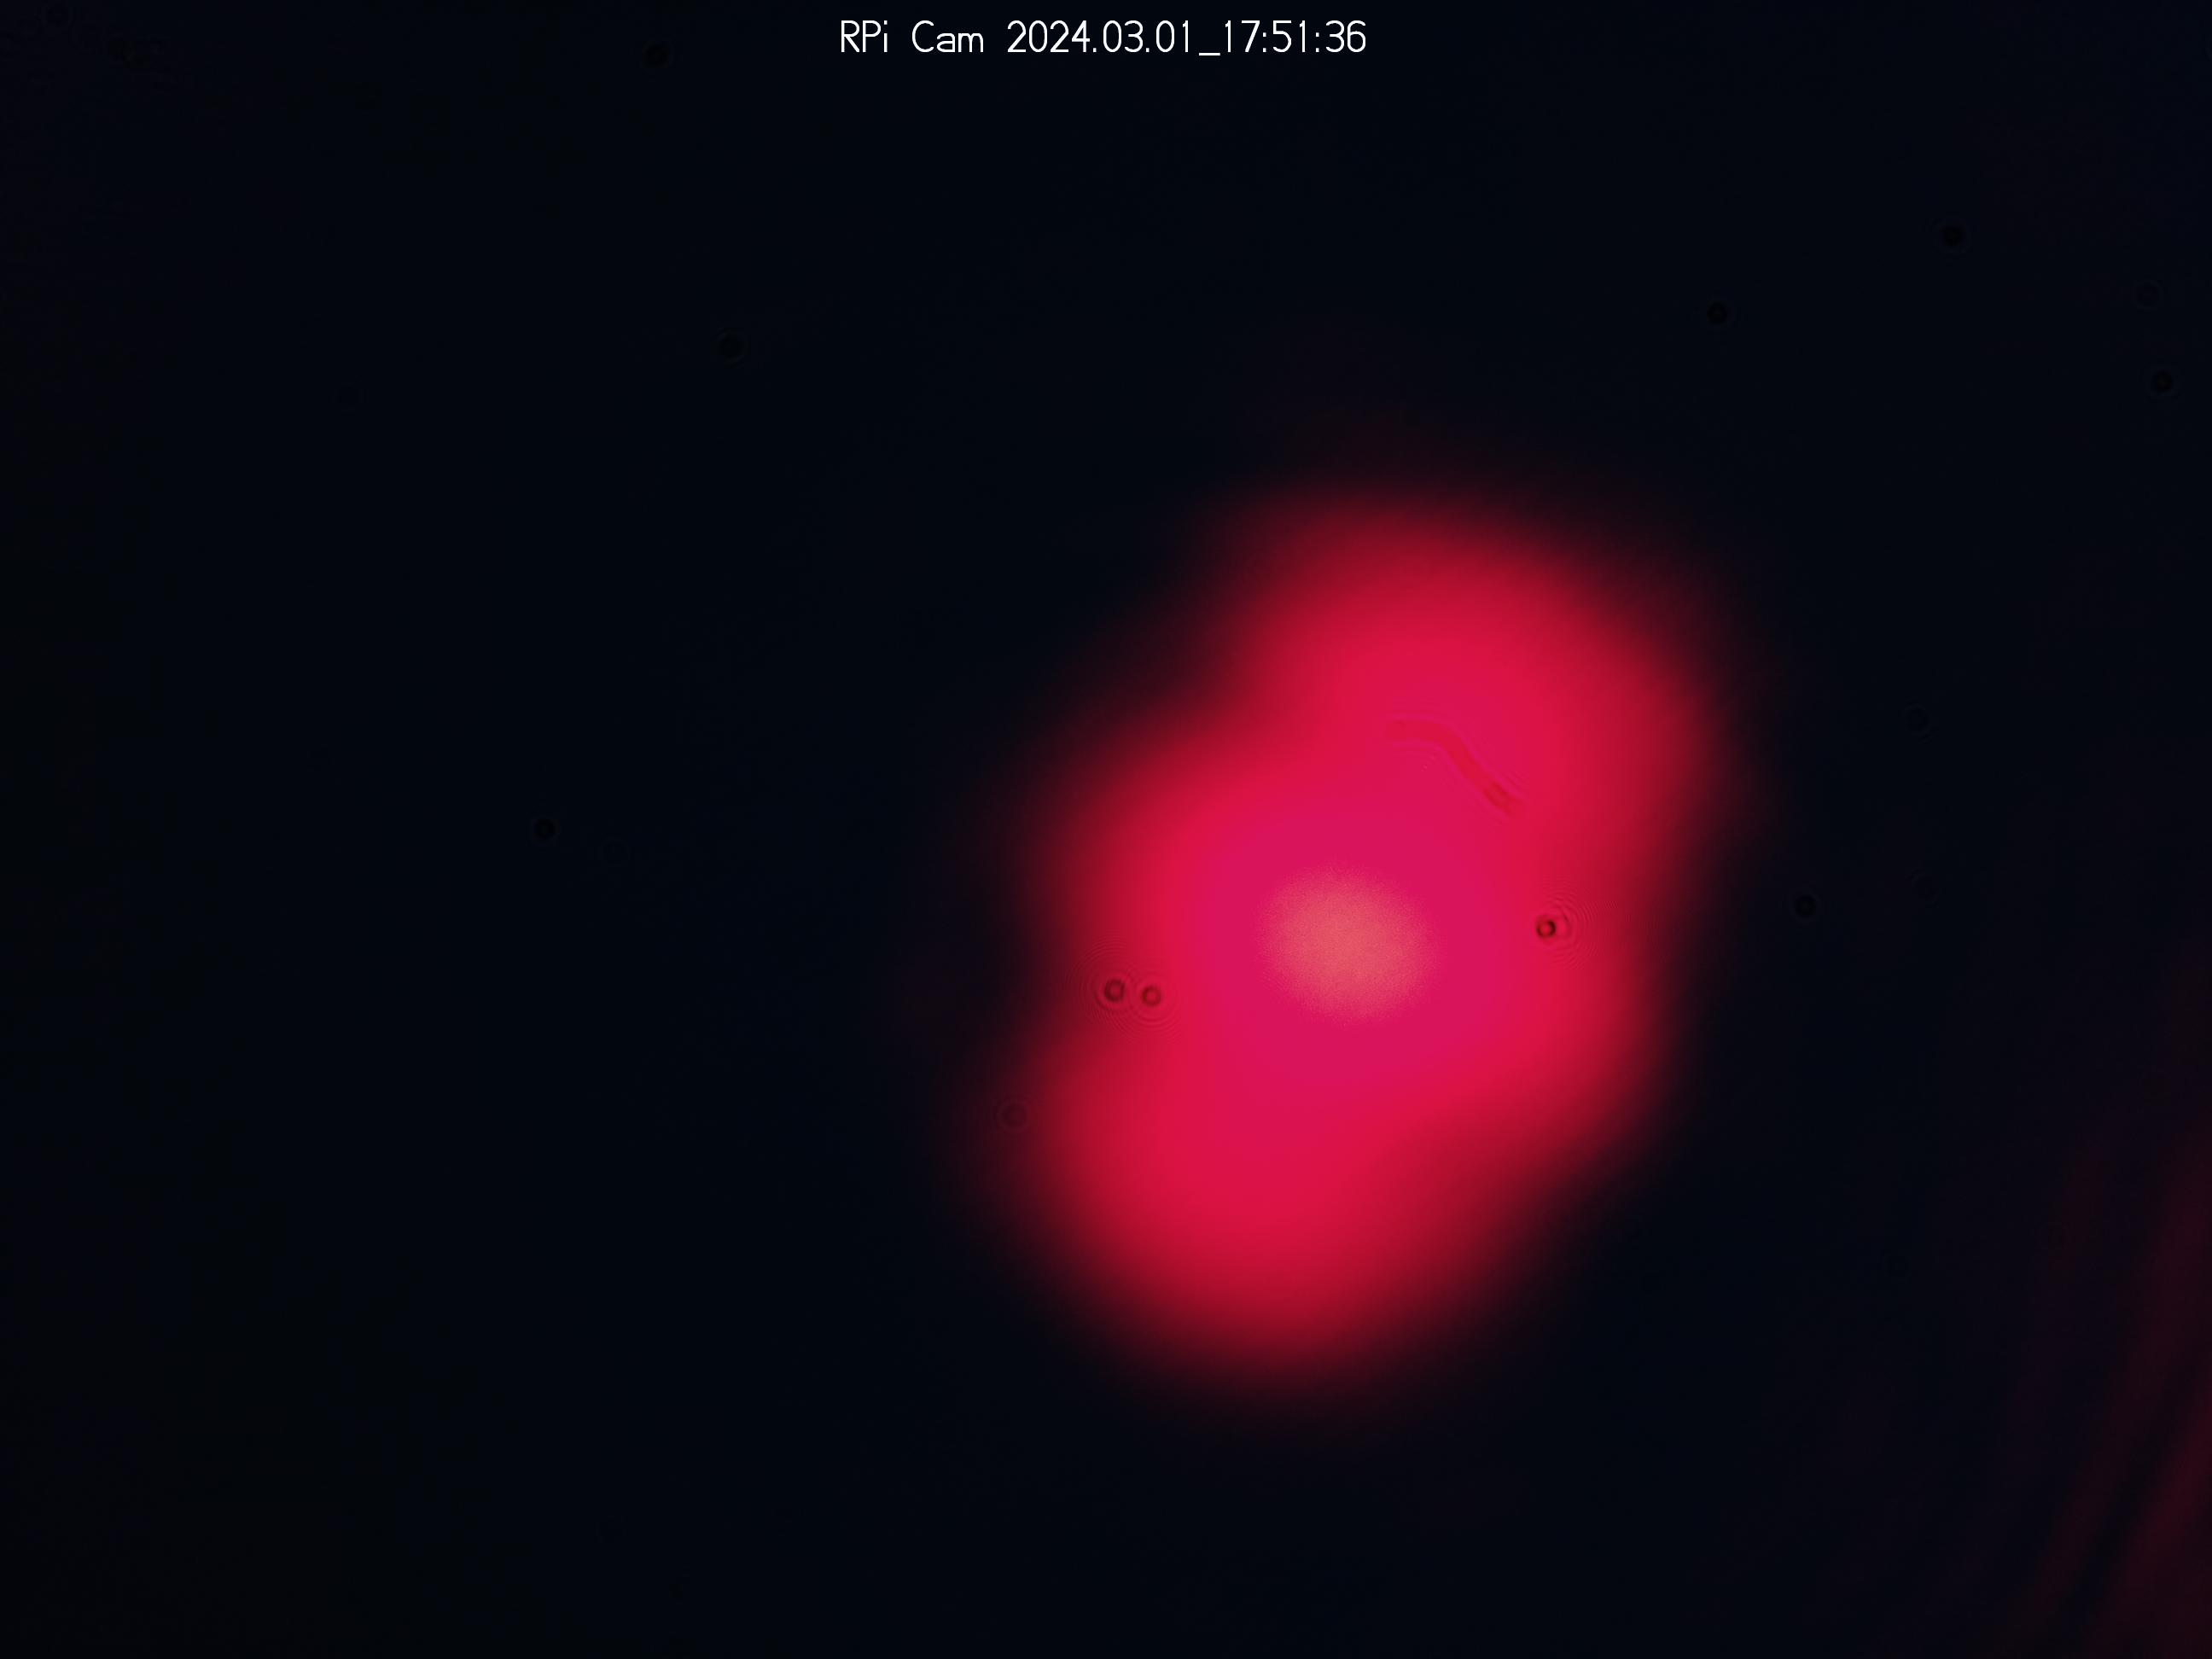
\includegraphics[width=0.3\textwidth]{data/2B/im_0227_20240301_175136.jpg}
    \includegraphics[width=0.3\textwidth]{data/2B/im_0228_20240301_175138.jpg}
    \caption{Intensity distributions for question 2.3.2B, from left to right starting from a complex mode as we close the iris. As the higher modes get cut off they stop lasing, and by the end only the TEM$_{00}$ mode is left.}
    \label{fig:2B}
\end{figure}

\noindent \textcolor{blue}{2.3.2i.} Generally we see only one mode at once, although occasionally there were definitely more complex shapes. This can be explained by the same reasoning as the previous question. The nature of the gain of a given mode occurs exponentially as more photons are emitted at that frequency, which means that once a given node dominates it will usually suppress all the others.

\noindent \textcolor{red}{2.3.2B and C.} When the wire was inserted, we observed the following modes as we moved the wire slowly across the range: TEM$_{00}$, TEM$_{30}$, TEM$_{20}$, TEM$_{10}$, TEM$_{20}$, TEM$_{00}$. This is expected for the exact same reason as what we saw in 2.2B. The wire blocks a certain part of the lasing to happen. If a given node has a nonzero brightness at the point the wire blocks, then each time the light bounces in the cavity some of it will be lost and lasing won't occur at that mode. In the center we see TEM$_{10}$ since that's dark in the middle for example, and at the edges we see TEM$_{00}$ since that's dark at the edges. It's not entirely clear why we see TEM$_{30}$ only on one side (we repeated a few times to make sure it wasn't just that we were moving the wire too fast). It's probably due to slight misalignment of the mirror, as this has a large effect on which modes can resonate. Also they're all $m=0$ modes because the wire's vertical position blocks the large portion of the light in the $m$ axis regardless of what mode is present. See table \ref{tab:2C} for the results in a table.

\begin{table}[htpb]
    \centering
    \caption{Table for question 2.3.2C. These are the positions of the wire at which each mode was seen. These were taken when the cavity mirrors were 62cm apart and the wire was 47.5cm from the end of the cavity.}
    \label{tab:label}
    \begin{tabular}{|c|c|}
    \hline
    Mode&Distance (mm)\\
    \hline
    00&7.32\\
    20&7.62\\
    10&7.8\\
    20&7.94\\
    30&8.1\\
    00&8.43\\
    \hline
    \end{tabular}
\end{table}

\noindent \textcolor{red}{2.3.2E.} We can assume that the 10 mode occurs in the middle which is at $7.8$cm. From equation 3.3-12 from Saleh and Teich, the 20 mode's intensity is proportional to $\mathbb G_{2}\left(\frac{\sqrt{2}x}{w(z)}\right)$. The place where this mode is apparent with wire is when this expression is zero, so using $\mathbb G_2$'s definition:
\[
\mathbb G_2(u)=(4u^2-2)e^{-u^2 /2}=0\implies u=\frac{1}{\sqrt{2}}\implies w(z_{\text{wire}})=2x=2\left( 7.8-7.62 \right) =0.36\text{mm}
.\]

\noindent \textcolor{red}{2.3.2F.} From equation 11.2-15 from Saleh and Teich:
\[
z_0^2= \frac{-d(R_1+d)(R_2+d)(R_2+R_1+d)}{\left( R_2+R_1+2d \right) ^2}\implies z_0\implies z_0=21.7\text{cm}
.\]
Similarly from 11.2-14, where $z_1$ is the coordinate of the HR mirror relative to the focus (expected to be negative):
\[
z_1= \frac{-d(R_2+d)}{R_2+R_1+2d}\implies z_1=-11.3
.\]

\noindent \textcolor{red}{2.3.2G.} The wire taken at 47.5cm from the HR mirror, so $z_\text{wire}=34.4$. Calculating for $w(z_{\text{wire}})$.
\[
w(z)=\sqrt{\frac{\lambda z_0}{\pi}\left( 1+\left( \frac{z}{z_0} \right) ^2 \right) }=0.39\text{mm}
.\]
This is very close to the 0.36mm we experimentally found previously. An small discrepancies probably come from the range of values where the modes were visible. For example for the 10 mode there was around 0.2mm of turning the micrometer that the mode was visible. Since we only turned the micrometer in one direction to avoid backlash it was hard to choose the exact middle of when it was visible, so this likely explains any discrepancy.

\noindent \textcolor{red}{2.3.3A.} The beam being polarized means that the electric field for all light in the laser is pointing in the same direction as the light propagates. Using the polarizer, we found that the laser is completely polarized. By rotating the polarizer, there was one angle that resulted in no light going through, and at 90$^{\circ}$ from this angle the (subjective) maximum light was let through.

\noindent \textcolor{red}{2.3.3B.} It is expected that the laser is polarized. When stimulated emission happens, the resulting photon is exactly identical to the photon that stimulated the original emission. This includes polarization, so whatever photons end up dominating the lasing process will all have the same polarization.

\noindent \textcolor{red}{2.3.4A.} See figure \ref{fig:4A}. The peaks don't react the same, only three peaks show large noticeable differences. The peaks that change are at approximately 594.5nm, 607.4nm and 609.5nm. These peaks will be investigated more thoroughly shortly.

\begin{figure}[htpb]
    \centering
    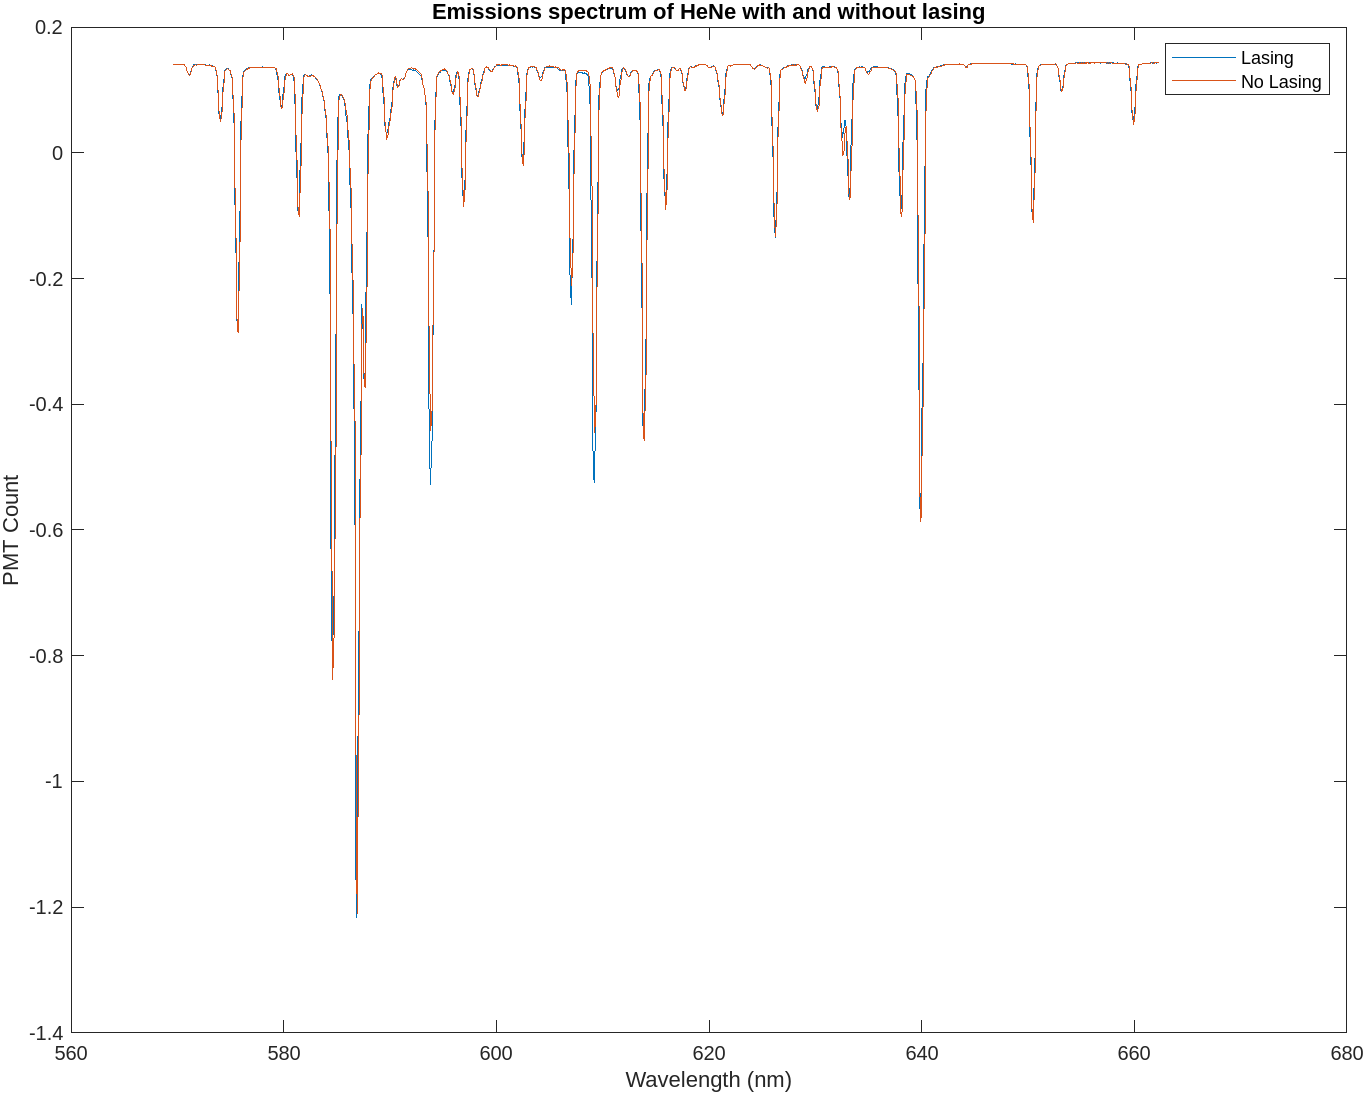
\includegraphics[width=0.8\textwidth]{4A}
    \caption{Graph for question 2.3.4A. This is the spectogram of the HeNe gas with and without lasing occuring. The spectrum is almost identical, except for a few specific peaks. These peaks with significant changes are at approximately 593.8nm, 607nm and 609.1nm.}
    \label{fig:4A}
\end{figure}

\noindent \textcolor{red}{2.3.4B.} See figure \ref{fig:4B}. 

\begin{figure}[htpb]
    \centering
    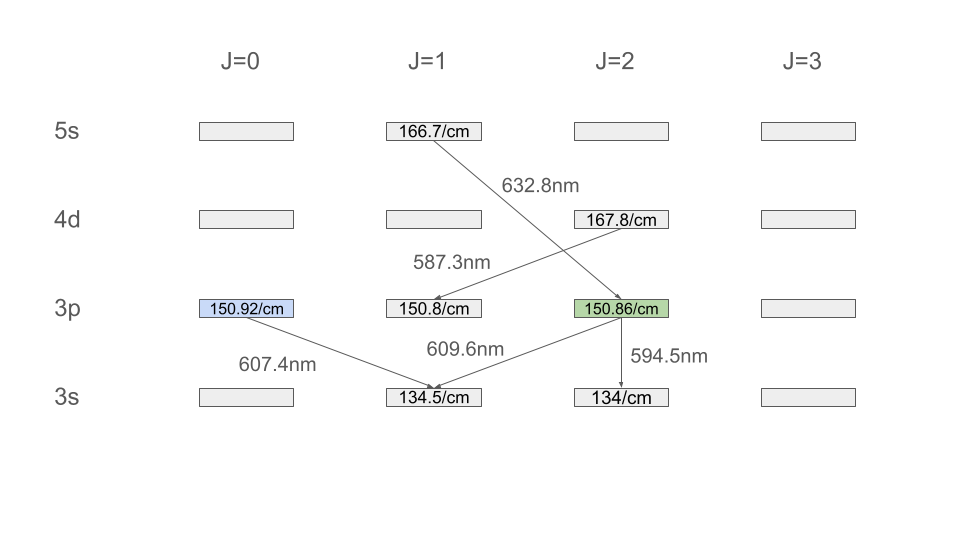
\includegraphics[width=0.8\textwidth]{4B}
    \caption{Diagram for question 2.3.4B. These are the transitions for HeNe. The number inside the level boxes is the energy of that state, while the nm in the arrows is the wavelength of the photon emitted for those levels. The 587.3nm is the largest peak in the spectorgram. The 632.8nm transition is shown, along with three others that share similar energy levels with it. 594.5 and 609.6nm (green) share the exact same spectrum, while 607.4nm (blue) shares an extremely close energy level, which is why experimentally we also see a change at that peak in figure \ref{fig:4A}.}
    \label{fig:4B}
\end{figure}

\noindent \textcolor{red}{2.3.4C.} See figure \ref{fig:4C}. We only see one laser line, corresponding to the 632.8nm transition we saw previously in figure \ref{fig:4B}. This makes sense, since by the nature of stimulated emission, all of the resulting photons will be at the same frequency. Thus only one laser line at a specific frequency will be seen

\begin{figure}[htpb]
    \centering
    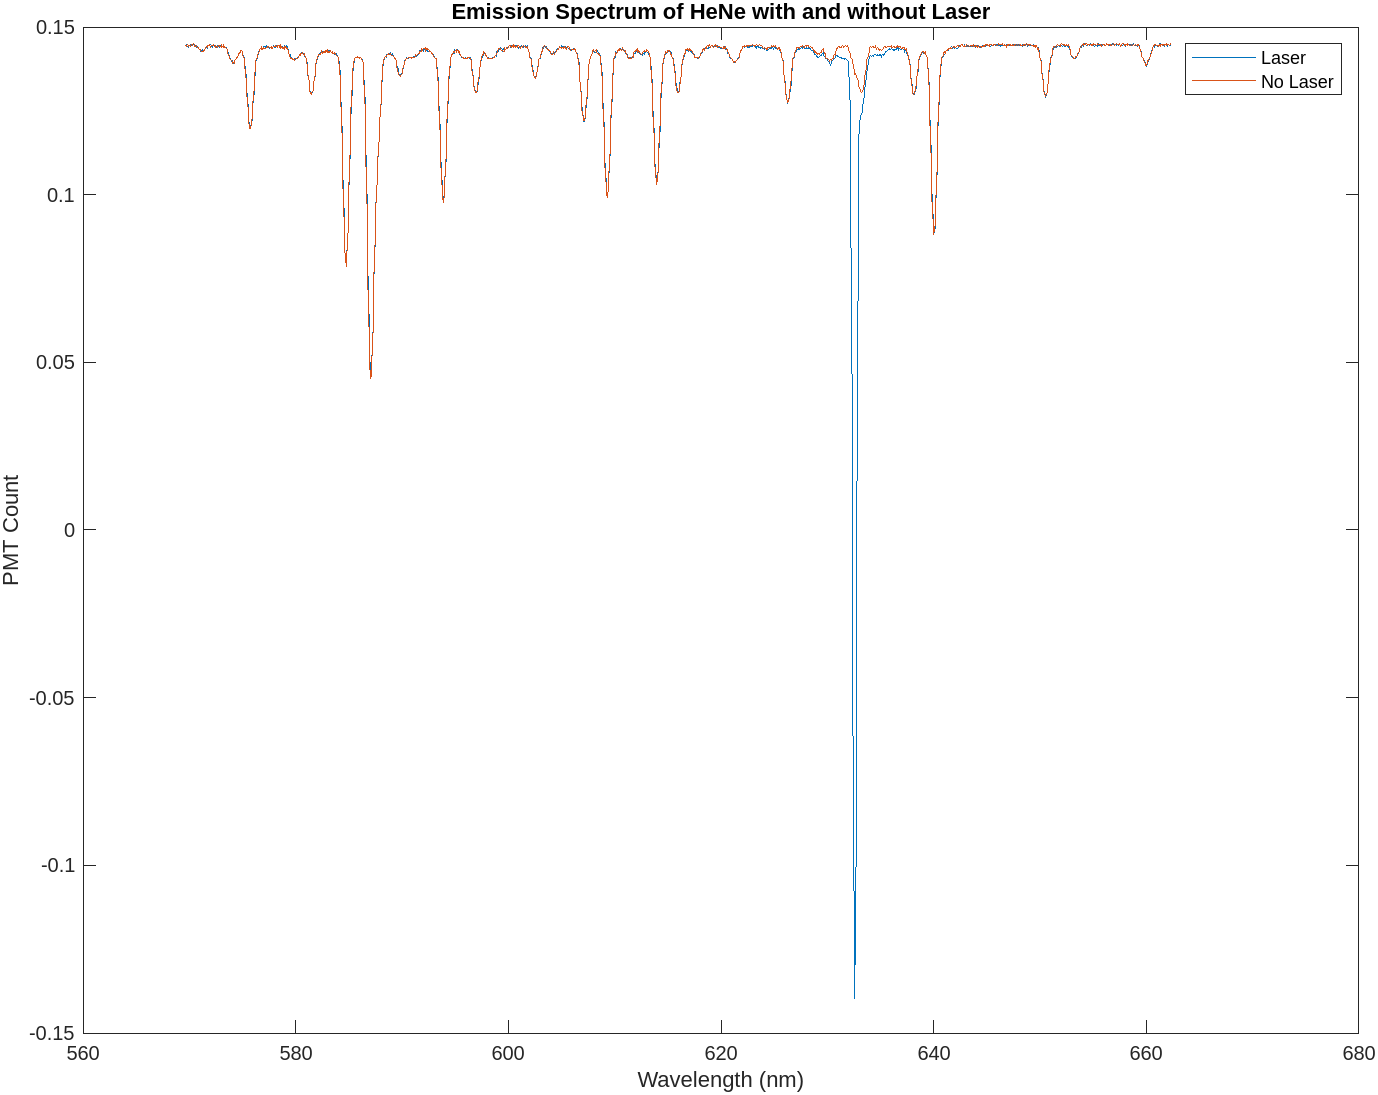
\includegraphics[width=0.8\textwidth]{4C}
    \caption{Graph for question 2.3.4C. This is the emission spectrum of the HeNe with and without the laser directly being diffused into the monochromator. The large laser line is the frequency that the laser is lasing at.}
    \label{fig:4C}
\end{figure}

\noindent \textcolor{blue}{2.3.4i.} The lasing line does not correspond to the largest fluorescence peak. The frequency that the light lases from is driven by the state that population inversion at occurs that, so there's no reason to think that the lasing peak would also happen to be the largest fluorescence peak.

\noindent \textcolor{red}{2.3.4D.} We set the chopper to 120Hz. The phase at which zero occurs is 320 degrees. Flipping by 180 degrees does nothing, the signal is still 0. The maximum signal is found at 50 degrees which is 90 degrees from the zero found previously, and flipping the phase from the maximum just flips the sign of the signal (which gives the minimum). The 90 degree difference between the zero and the max can be easily seen from the basics of op-amp function, since the signal is modulated by $\sin(\omega t+\phi)$. The op-amp averages this signal, so assuming that the input signal is $\sin(\omega t+\psi)$, the output of the op amp is
\[
\frac{1}{T}\int_{0}^{T}\sin(\omega t+\phi)\sin(\omega t+\psi)dt
.\]
This integral has a maximum when $\phi$ and $\psi$ are in phase and is zero when $\phi$ and $\psi$ are 90 degrees offset, perfectly explaining the observed behavior.

\noindent \textcolor{red}{2.3.4E.} The sign of the lock in amplifier did change sign. This is entirely expected. Before we removed blocked the laser, the line at 632.8nm was incredibly strong from the laser. In contrast, when the laser is blocked we're looking at the difference in spontaneous emission at 632.8nm between lasing and no lasing. This has the opposite effect, of where during lasing no spontaneous emission can occur at 632.8nm because all Ne atoms that could spontaneously emit are undergoing stimulated emission instead. Note that the magnitude of this effect is much smaller than the laser directly pointed at the monochromator, and this is seen by the lock in as a much smaller magnitude of its output signal.

\noindent \textcolor{red}{2.3.4F.} See figure \ref{fig:4F}. The lock-in output is proportional to the difference between the on and off lasing state of the HeNe. This is a much lower noise measurement than just subtracting them if we were to do so in part 2.3.4F. This confirms the results of part 2.3.4B, as the affected lines are at almost the exact frequencies we saw in figure \ref{fig:4B}: 594.5nm, 607.4nm and 609.6nm. The reason that these lines are modulated is that, as the hint suggests, the stimulated emission causes many more emissions at the 632.8nm level, the result of which is many more atoms at energy levels amenable to spontaneous emission at the frequencies just listed.

\begin{figure}[htpb]
    \centering
    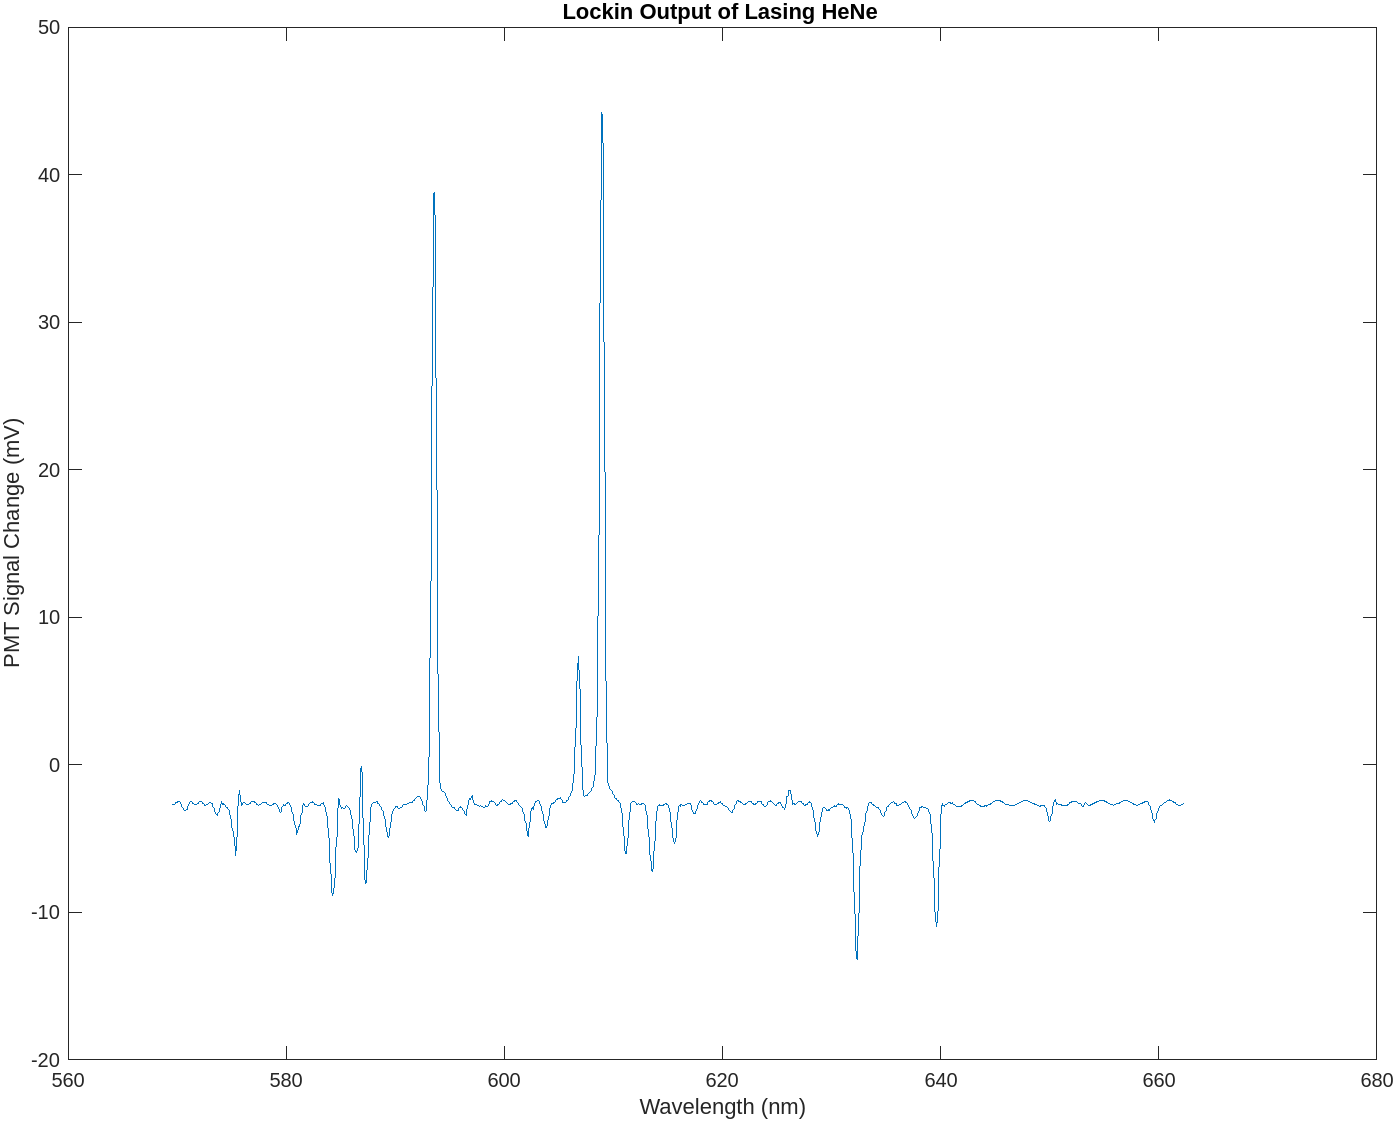
\includegraphics[width=0.8\textwidth]{4F}
    \caption{Lock-in output for question 2.3.4F. The three peaks that occur are almost exactly the peaks identified earlier in part 2.3.4A.}
    \label{fig:4F}
\end{figure}

\end{document}
